\documentclass[12pt,letterpaper]{exam}

\newcommand{\DocTitle}{Renew the DocTitle variable.}
\newcommand{\CourseNumber}{NE555}
\newcommand{\CourseName}{Nuclear Reactor Dynamics}
\newcommand{\DayTime}{TuTh 8:00-9:15}
\newcommand{\Room}{VV\&E B129}
\newcommand{\Term}{Spring 2011}
\newcommand{\Instructor}{Lewis John Lloyd}
\newcommand{\School}{University of Wisconsin - Madison}

\usepackage{listings}
\usepackage{mathtools}
\usepackage{xtab}
\usepackage{longtable}
\usepackage{array}
\usepackage{mathrsfs}
\usepackage{color}
\usepackage{multicol}
\usepackage{pdflscape}
\usepackage{pdfpages}
\usepackage{graphicx}
\usepackage{esint}
\usepackage{amsmath}
\usepackage{amssymb}
\usepackage{graphics}

\usepackage[
			pdfborder={0 0 0},
			urlcolor=cyan,
			pdftitle={\CourseNumber \DocTitle},
			pdfauthor={\Instructor}
			]{hyperref}
			
\usepackage[
			includeheadfoot,
			top=0.5in,
			bottom=0.5in,
			left=1.0in,
			right=1.0in
			]{geometry}
\setlength{\parindent}{0in}
\setlength{\parskip}{\baselineskip}

\lhead{\CourseNumber: \CourseName}
\chead{}
\rhead{\Term}
\lfoot{}
\cfoot{\thepage}
\rfoot{}
\coverlhead{\CourseNumber: \CourseName}
\coverchead{}
\coverrhead{\Term}
\coverlfoot{}
\covercfoot{\School}
\coverrfoot{}


\correctchoiceemphasis{\bfseries\color{red}}
\bracketedpoints
\pointsinmargin
%\addpoints
%\shadedsolutions

\lstset{ %
language=Matlab,                % the language of the code
basicstyle=\footnotesize,       % the size of the fonts that are used for the code
numbers=left,                   % where to put the line-numbers
numberstyle=\footnotesize,      % the size of the fonts that are used for the line-numbers
stepnumber=5,                   % the step between two line-numbers. If it's 1, each line 
                                % will be numbered
numbersep=5pt,                  % how far the line-numbers are from the code
backgroundcolor=\color{white},  % choose the background color. You must add \usepackage{color}
showspaces=false,               % show spaces adding particular underscores
showstringspaces=false,         % underline spaces within strings
showtabs=false,                 % show tabs within strings adding particular underscores
frame=single,                   % adds a frame around the code
tabsize=2,                      % sets default tabsize to 2 spaces
}

\renewcommand{\solutiontitle}{\noindent\textbf{Solution:}\par\noindent}

\newcommand{\mathsym}[1]{{}}
\newcommand{\unicode}{{}}
\newcommand{\tr}[1]{\tilde{#1}}
\newcommand{\LapTran}[1]{\mathscr{L}\left[#1\right]}
\newcommand{\InvLapTran}[1]{\mathscr{L}^{-1}\left[#1\right]}
\newcommand{\ParDer}[2]{\frac{\partial #1}{\partial #2}}
\newcommand{\Der}[2]{\frac{d\; #1}{d\;#2}}


\renewcommand{\DocTitle}{Problem Set 03}
\noprintanswers

%-------------------------------------------------------------------------------------
\begin{document}
%-------------------------------------------------------------------------------------
\begin{center}
\textbf{\DocTitle}
\end{center}
%-------------------------------------------------------------------------------------
\textbf{NOTES}: 
Be sure to provide axis labels and legends for each plot.
Be sure to enclose your analytic solutions with boxes.
Be sure to provide a print out of computer code used during the problem set.
For all parts of this problem set, use the physical parameters on page 2.


\begin{questions}
%-------------------------------------------------------------------------------------
\question[20]{
On the webpage, there is a link to 'power.csv.'
Download this file.
In the file you will find two columns of data.
The two columns provide a time [ms] and power [kW] for a test reactor during a transient.
Using a program of your choice, determine the asymptotic period of this transient.
Using the Inhour equation for 6DG, estimate the constant reactivity insertion that would have created this power profile.
Using the Inhour equation for 1DG, estimate the constant reactivity insertion that would have created this power profile using the two forms of the 1DG decay constant specified in Problem 2.
Plot the data and $\displaystyle P(t)$ with the reactivities you obtained from the 6DG and the two 1DG reactivity approximations. 
Use the equations that correspond to the reactivity to plot the power (i.e., 6DG PRKE for the $\rho$ obtained from the 6DG Inhour Equation).
Comment on your plots.
\fullwidth{\begin{solution}
Using all data points results in an asymptotic period of $\displaystyle \alpha\,\simeq 0.0107\,[\,\frac{1}{s}\,]$.
If you chopped some of the initial jump data, you will get a slightly lower value.
Using the 6DG Inhour equation,
$$\displaystyle \rho = \alpha\left(\,\Lambda\,+\,\sum_{k=1}^{6}\frac{\beta_k}{\alpha+\lambda_k}\right)$$,
we get $\displaystyle \rho_{6GD} \simeq 6.77\cdot 10^{-04} [-]$.
Using the 1DG Inhour equation,
$$\displaystyle \rho = \alpha\left(\,\Lambda\,+\,\sum_{k=1}^{6}\frac{\beta_k}{\alpha+\lambda_k}\right)$$,
we get $\displaystyle \rho_{inv} \simeq 7.95\cdot 10^{-04} [-]$ and $\displaystyle \rho_{ave} \simeq 1.67\cdot 10^{-04} [-]$.
These values respectively correspond to the use of $\bar{\lambda}_{inv}$ and $\bar{\lambda}_{ave}$ as the 1DG decay constants.

Comments may vary.

Graphs at end of solution.
\end{solution}}}
\ifprintanswers
\pagebreak
\fi
%-------------------------------------------------------------------------------------
\question{
Consider a reactivity insertion of $\rho$ = $\displaystyle\frac{\beta}{10}$ at t = 0 [s].
Prior to this insertion, the reactor has been operating at steady state for a long time.
Neglect the source term in this problem.
\begin{parts}
\part{
Produce plots of the power of the reactor versus time for 30 [s] using the following forms of the one delayed neutron group decay constant:
\begin{subparts}
\subpart[5]{
$$ \lambda = \frac{\displaystyle \sum_{k\, =\, 1}^{6}\,\lambda_k\,\beta_k}{\displaystyle \sum_{k\,=\,1}^{6}\,\beta_k}$$
\fullwidth{\begin{solution}
$$\displaystyle \lambda = 0.4054 [\frac{1}{s}]$$
Graph at end of solution.
\end{solution}}
}
\subpart[5]{
$$ \lambda = \frac{\displaystyle \sum_{k\, =\, 1}^{6}\,\beta_k}{\displaystyle \sum_{k\,=\,1}^{6}\,\frac{\beta_k}{\lambda_k}}$$
\fullwidth{\begin{solution}
$$\displaystyle \lambda = 0.0767 [\frac{1}{s}]$$
Graph at end of solution.
\end{solution}}
}
\end{subparts}
}
\part[15]{
Use a computer to numerically evaluate the six delayed neutron group PRKE out to t = 30 [s].
Matlab has many built-in solvers such as ode45 and ode15s which will make this an easy task.
Provide a plot of the power of the reactor versus time for 30 [s].
\fullwidth{\begin{solution}
Graph at end of solution.
\end{solution}}
}
\part[5]{
Comment on the maximum power achieved by each method. 
What are your thoughts on the differences between the three plots?
\fullwidth{\begin{solution}
Comments may vary.
\end{solution}}
}
\part[10]{
Use Laplace Transforms to obtain a symbolic solution for the power using the one delayed neutron group PRKE.
Show all of your work for full credit.
Do \textbf{NOT} use a software algebra solver such as Mathematica to do this.
\fullwidth{\begin{solution}
\begin{multicols}{2}
Laplace Transform both equations.
\begin{eqnarray*}
\LapTran{\frac{dp}{dt}} & = & \left[\frac{\rho-\beta}{\Lambda}\right]\,\LapTran{p}+\frac{\lambda}{\Lambda}\LapTran{c}\\
\LapTran{\frac{dc}{dt}} & = & -\lambda\,\LapTran{c}+\beta\,\LapTran{p}\\
s\,\tr{p} - p(0) & = & \left[\frac{\rho-\beta}{\Lambda}\right]\,\tr{p}+\frac{\lambda}{\Lambda}\tr{c}\\
s\,\tr{c} - c(0) & = & -\lambda\,\tr{c}+\beta\,\tr{p}\\
\end{eqnarray*}
Solve for $\tr{c}$ in terms of $\tr{p}$.
\begin{eqnarray*}
s\,\tr{c} - c(0) & = & -\lambda\,\tr{c}+\beta\,\tr{p}\\
s\,\tr{c} +\lambda\,\tr{c} & = & c(0)+\beta\,\tr{p}\\
\tr{c}(s +\lambda) & = & \frac{\beta}{\lambda}p(0)+\beta\,\tr{p}\\
\tr{c} & = & \frac{\beta}{\lambda}\frac{p(0)}{(s +\lambda)}+\beta\,\frac{\tr{p}}{(s +\lambda)}\\
\end{eqnarray*}
Eliminate $\tr{c}$ from the equation for $\tr{p}$ and solve for $\tr{p}$.
\begin{eqnarray*}
s\,\tr{p} -\left[\frac{\rho-\beta}{\Lambda}\right]\,\tr{p}-\frac{\lambda}{\Lambda}\tr{c} & = & p(0)\\
\tr{p}(s-\left[\frac{\rho-\beta}{\Lambda}\right]-\frac{\lambda\beta}{\Lambda(s+\lambda)})& = & \\
p(0)(1+\frac{\beta}{\Lambda(s+\lambda)}) & &\\
\end{eqnarray*}
\begin{eqnarray*}
\frac{\tr{p}}{p(0)} & = &(\frac{\lambda+\frac{\beta}{\Lambda}+s}{s^2+s\,(\lambda-\frac{\rho-\beta}{\Lambda})-\frac{\lambda\,\rho}{\Lambda}})\\
& = & \frac{\lambda+\frac{\beta}{\Lambda}+s}{(s-\omega_1)(s-\omega_2)}\\
\end{eqnarray*}
Using $\displaystyle\rho\, =\,\frac{\beta}{10}$, $\omega_{1,2}$ are defined as:
\begin{eqnarray*}
\omega_{1,2} & = & -\frac{9\beta+10\lambda\Lambda}{20\Lambda}\\
& \pm & \frac{\sqrt{81\beta^2+220\beta\lambda\Lambda+(10\lambda\beta)^2}}{20\Lambda}\\
\gamma & = &\frac{9\beta+10\lambda\Lambda}{20\Lambda}\\
\delta & = & \frac{\sqrt{81\beta^2+220\beta\lambda\Lambda+(10\lambda\beta)^2}}{20\Lambda}\\
\omega_{1,2} & = & -\gamma \pm \delta\\
\end{eqnarray*}
Apply the Inverse Laplace Transform.
\begin{eqnarray*}
\frac{p(t)}{p(0)} & = & \InvLapTran{\frac{\lambda+\frac{\beta}{\Lambda}+s}{(s-\omega_1)(s-\omega_2)}}\\
\frac{p(t)}{p(0)} & = & \frac{\lambda+\frac{\beta}{\Lambda}+\omega_1}{\omega_1-\omega_2}e^{\omega_1\,t}\\
&+&\frac{\lambda+\frac{\beta}{\Lambda}+\omega_2}{\omega_2-\omega_1}e^{\omega_2\,t}\\
\frac{p(t)}{p(0)} & = & \frac{e^{-\gamma\,t}}{2\delta}\left[e^{\delta\,t}(\lambda+\frac{\beta}{\Lambda}-\gamma+\delta)\right]\\
&-&\frac{e^{-\gamma\,t}}{2\delta}\left[e^{-\delta\,t}(\lambda+\frac{\beta}{\Lambda}-\gamma-\delta)\right]\\
\end{eqnarray*}
With:
\begin{eqnarray*}
\gamma & = &\frac{9\beta+10\lambda\Lambda}{20\Lambda}\\
\delta & = & \frac{\sqrt{81\beta^2+220\beta\lambda\Lambda+(10\lambda\beta)^2}}{20\Lambda}\\
\xi & = & \frac{\lambda+\frac{\beta}{\Lambda}-\gamma}{\delta}
\end{eqnarray*}
The solution is:
$$\displaystyle p(t) = p(0)\,e^{-\gamma\,t}\left[cosh(\delta\,t)+\xi\,sinh(\delta\,t)\right]$$
\end{multicols}
\vfill
\end{solution}}
}
\end{parts}}
%-------------------------------------------------------------------------------------
\end{questions}
\pagebreak
\begin{center}
\setlength{\extrarowheight}{2.0pt}
\begin{tabular}{lcc}
Group & $\lambda_k$ [1/s] & $\displaystyle \frac{\beta_k}{\beta}$ [-] \\ \hline
1 & 0.0124 & 0.033	\\
2 & 0.0305 & 0.219	\\
3 & 0.1110 & 0.196	\\
4 & 0.3010 & 0.395	\\
5 & 1.1400 & 0.115	\\
6 & 3.0100 & 0.042	\\
\end{tabular}
\end{center}

$\beta$ = 0.00650 [-] \\
$\Lambda$ = 7.6427e-06 [s]

\ifprintanswers
\begin{landscape}
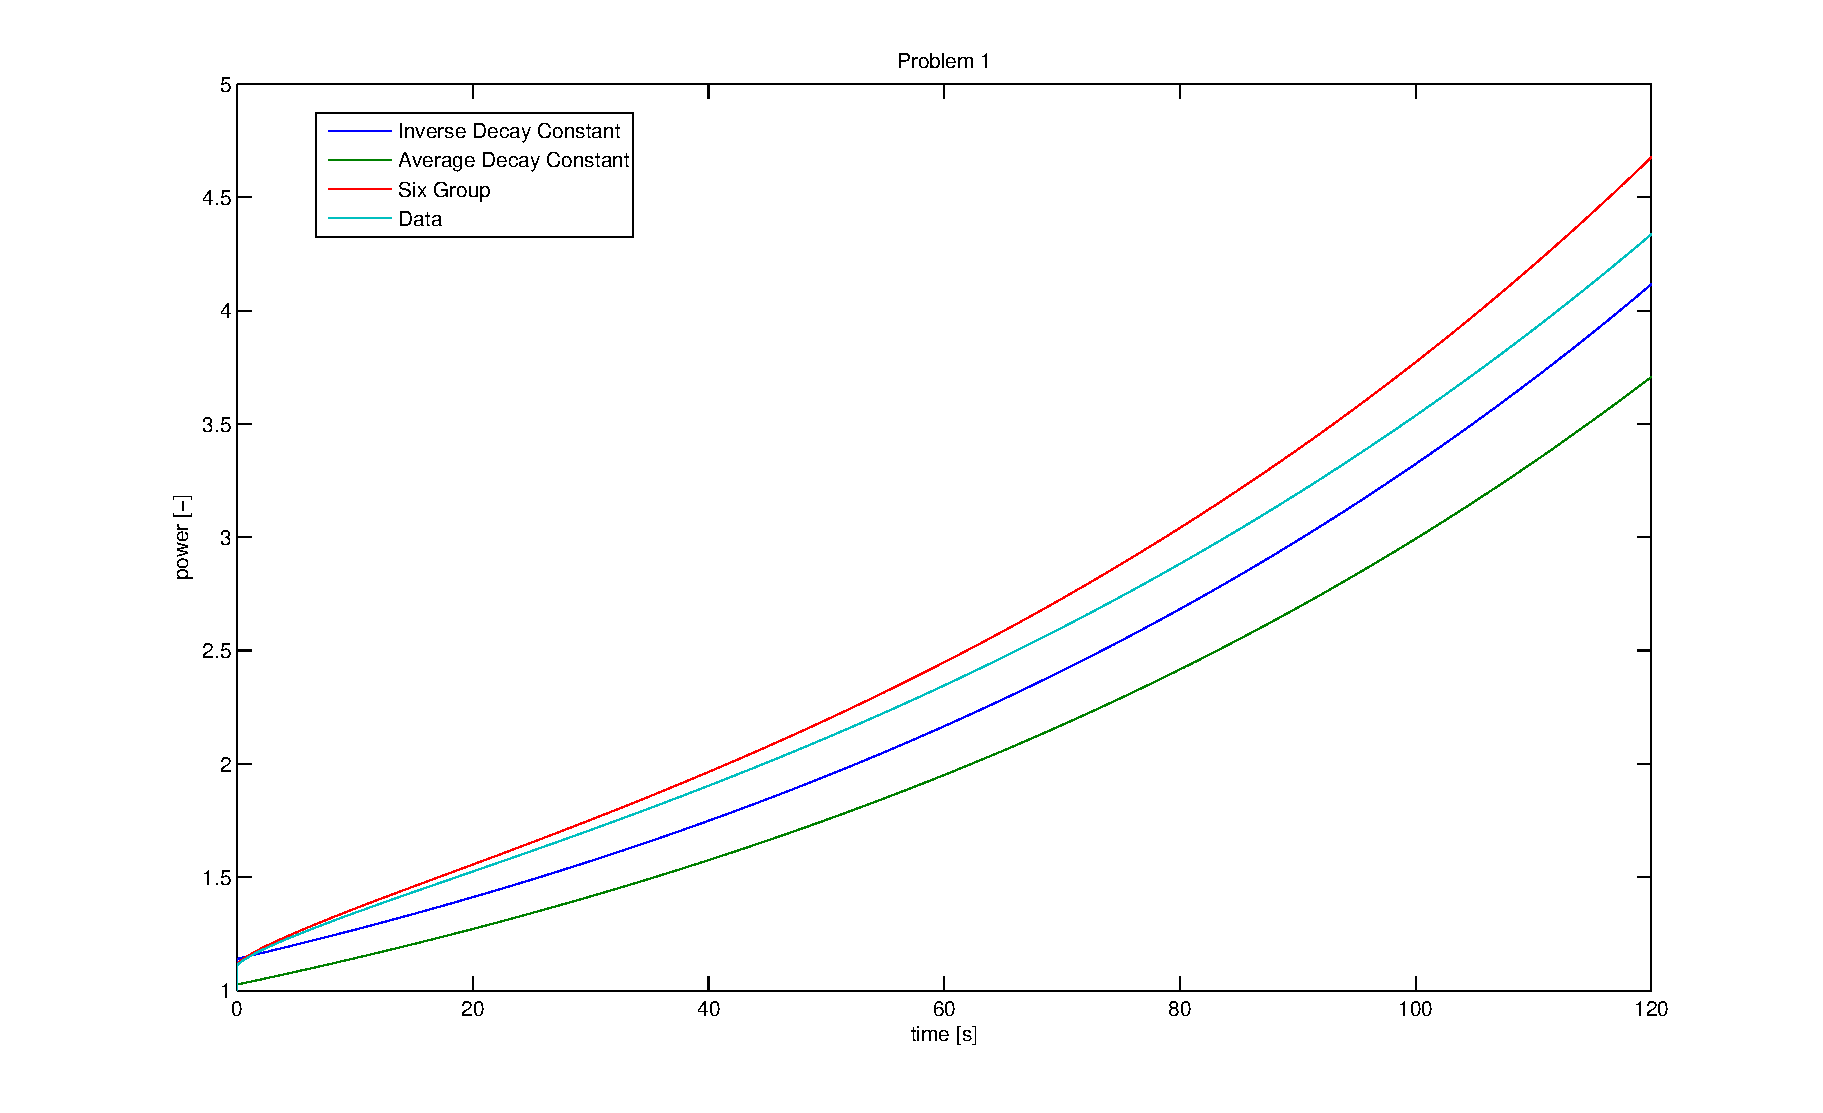
\includepdf[landscape=true]{PS03Q01pic.pdf}
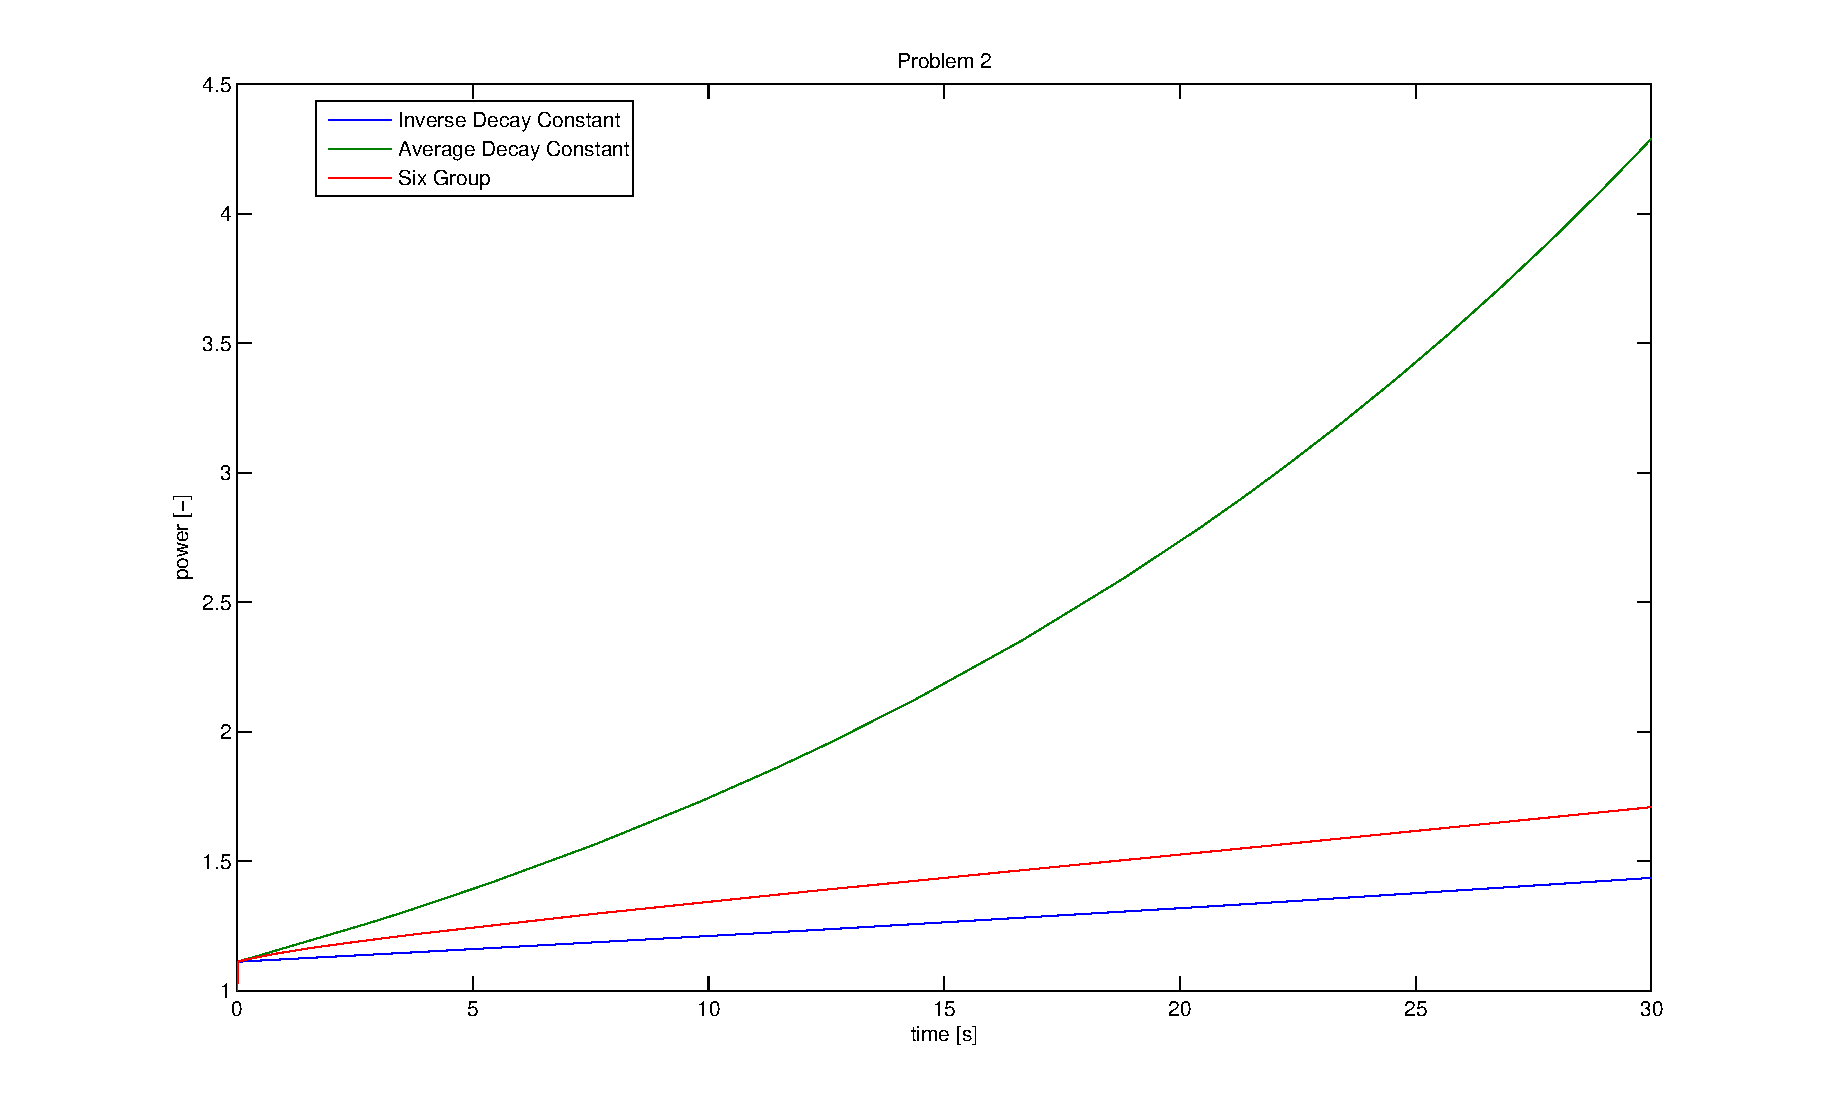
\includepdf[landscape=true]{PS03Q02pic.pdf}
\end{landscape}
\fi

\end{document}